\begin{titlepage}

	\centering
    \vspace*{0.5 cm}
	\rule{\linewidth}{0.2 mm} \\[0.4cm]
	\begin{spacing}{1.1}
		\huge \bfseries Fire Services by Project-alias\\[0.3cm]
		\LARGE User Manual
	\end{spacing}
	\rule{\linewidth}{0.2 mm} \\[1 cm]


	\textsc{\large $Demo 0.1$}\\[4cm]

	% uncomment the following block to add a logo
	% \begin{center}
	% \includegraphics[height=4cm]{sections/00-toc/images/logo.pdf}
	% \end{center}

 
	\vfill
	\noindent
	\begin{minipage}{0.7\textwidth}
		\begin{flushright}
			\textsc{Project:}\\
			\textsc{Draft Date:}\\
		\end{flushright}
	\end{minipage}~~\hspace*{1 cm}
	\begin{minipage}{0.3\textwidth}
		\begin{flushleft}
			fire_services\\
			2022.01.02\\
		\end{flushleft}
	\end{minipage}

	\clearpage

	\setcounter{page}{1}
	\justifying
	The Project-alias fire system allows managing assets including Equipment and Vehicles available in Fire Services departments by tracking essential characteristics such as titles, activity status, descriptions, serial numbers, assigned drivers etc. Also, it allows efficient preventive maintenance task tracking through creating form templates and ability to fill them up. 
	
	\vspace{5mm}
	The Demo Application contains four modules that will be described in this manual: 
	\begin{enumerate}
  \item Equipment.
  \item Vehicle.
  \item Forms.
  \item Users and Personnel. 
\end{enumerate}
\vspace{5mm}
	\begin{center}
  \makebox[\textwidth]{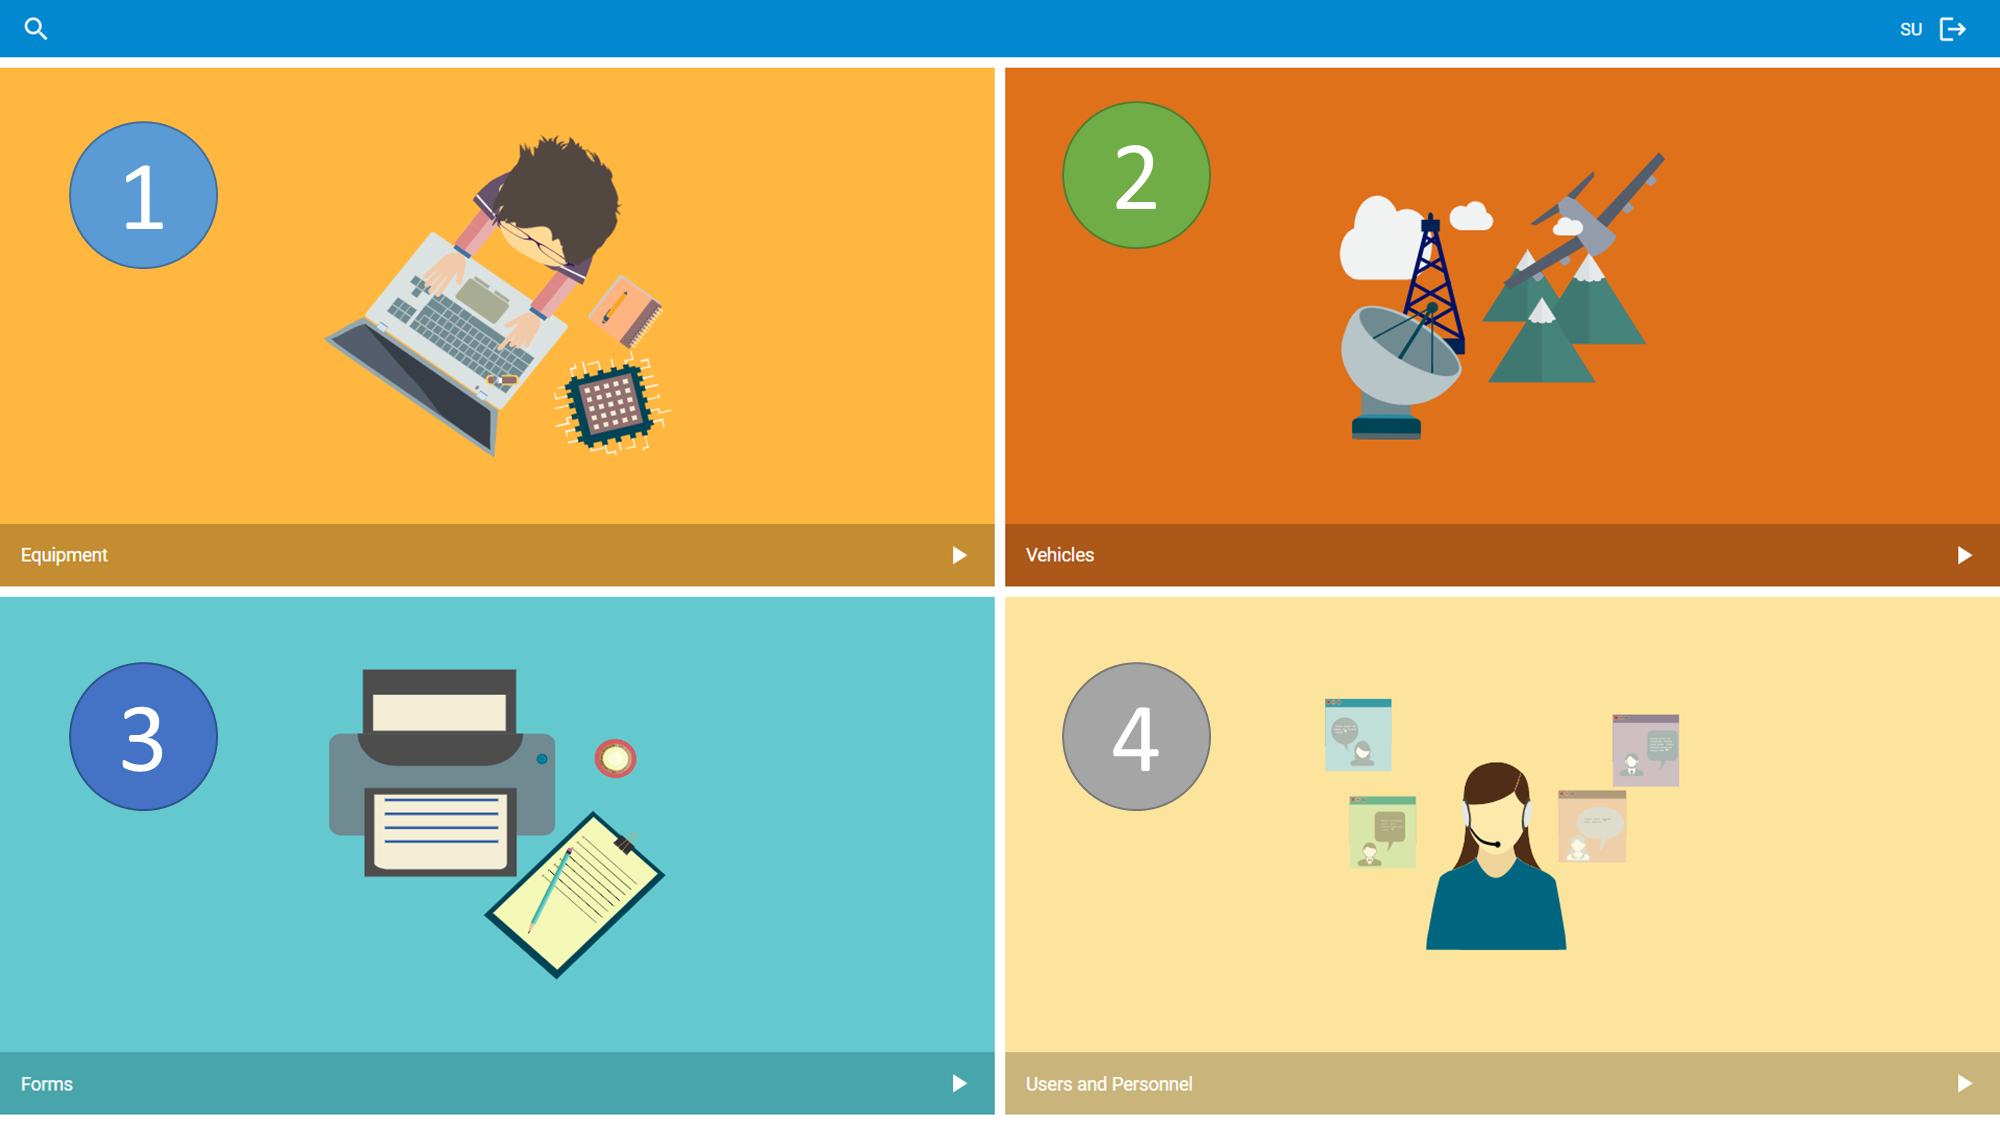
\includegraphics[width=1\textwidth]{sections/00-toc/images/main-menu.png}}
\end{center}

    \clearpage
	
    \setcounter{tocdepth}{3}
    \tableofcontents

    \clearpage

\end{titlepage}
